\chapter{Teori om filtre}
\label{TeoriOmFiltre}
Formålet med følgende afsnit er at afdække relevant teori i forhold til at designe et filter, der tilfredsstiller opgavens formål på bedst mulig vis. Opbygningen af et elektronisk filter med henblik på hvilke komponenter, der skal benyttes vil blive afdækket, samt hvad man kan opnå ved at veksle mellem disse.

\section{Komponenter}
\label{Komponenter}
Når man beskæftiger sig med elektroniske kredsløb skelner man hovedsagligt mellem aktive og passive komponenter. Forskellen på disse er, hvorvidt en komponents funktion
\subsection{Modstand}
\label{Modstand}

\input{Content/Teori/TeoriOmFiltre/Kondensator}
\section{Test af filtre}
Filtrenes frekvensrespons er målt med et sinus-sweep for et enkelt filter ad gangen. På \autoref{fig:UdregnetKontraPraktiskGain} sammenlignes de fysiske, med de simulerede filtres frekvensrespons. Simuleringerne tager udgangspunkt i ideelle komponentværdier imens de fysiske komponenter kan have små afvigelser, jævnfør \fullref{TilpasningAfFilter}. Kurverne er nærmest identiske, hvilket er yderst tilfredsstillende.
%
\begin{figure}[H]
	\centering
	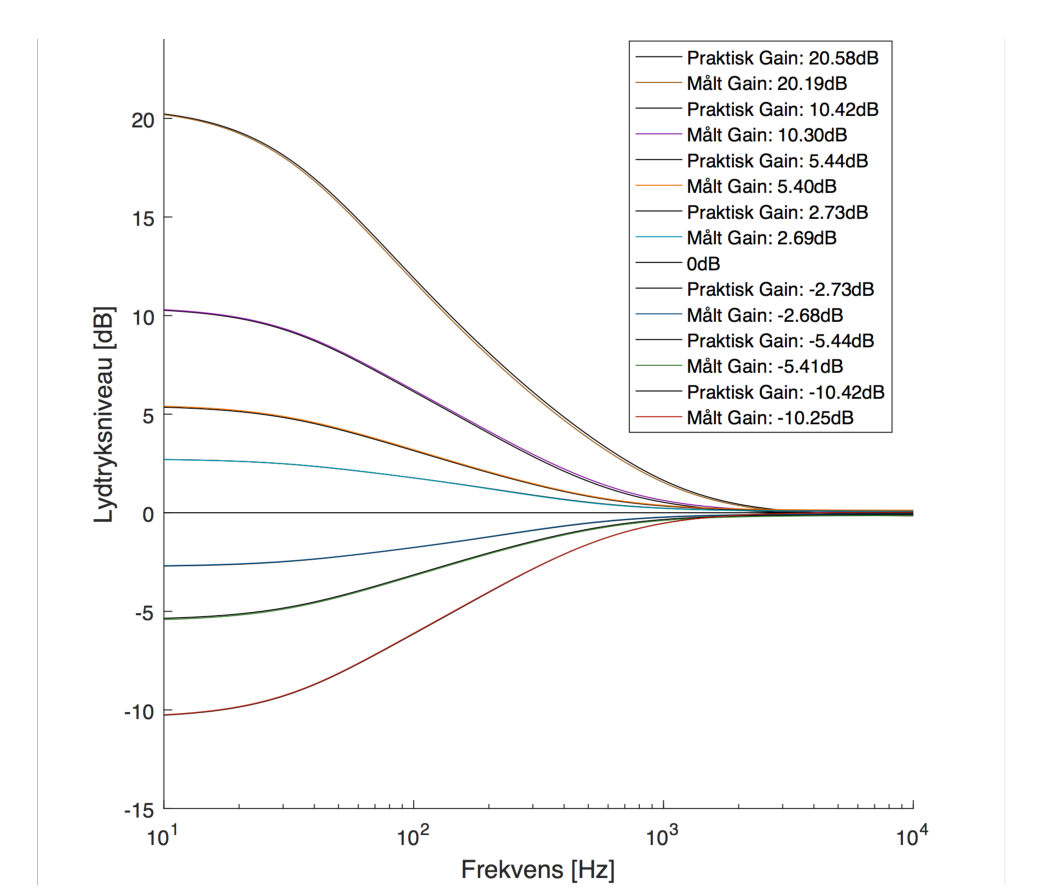
\includegraphics[resolution=300,width=\textwidth]{Figure/DesignAfFilter/PraktiskKontraSweepsSHORT.pdf}
	\caption{Frekvensrespons for simulerede filtre, sammenlignet med målte værdier af fysiske filtre.}
	\label{fig:UdregnetKontraPraktiskGain}
\end{figure}
\noindent
%
THD i de enkelte filtre er særdeles lavt. Dette er meget tilfredsstillende og langt under hvad der var forventet af filtrene. De respektive THD-værdier fremgår af \autoref{tab:THDFiltre}
%
\begin{table}[H]
\centering
\begin{tabular}{|l|l|l|l|l|l|l|l|}
\hline
Filter & 2.62 & 5.24 & 10.48 & 20.96 & -2.62 & -5.24 & -10.48 \\ \hline
THD \% & 0.0025 & 0.0024 & 0.0022 & 0.002 & 0.0027 & 0.0031 & 0.0031 \\ \hline
\end{tabular}
\caption{Sinus-sweep}
\label{tab:THDFiltre}
\end{table}


\input{Content/Teori/TeoriOmFiltre/Operationsforstaerker}
\input{Content/Teori/TeoriOmFiltre/Aktivefiltre}


\input{Content/Teori/TeoriOmFiltre/LogiskePorte}
\input{Content/Teori/TeoriOmFiltre/Multiplekser}
\input{Content/Teori/TeoriOmFiltre/Overfoeringsfunktion}




%\section{Filtertype: Aktive og Passive}
\label{Filtertype}
%\begin{itemize}
%  \item Aktivt eller passivt filter inklusiv komponenter
%  \item Fordele og ulemper
%  \item Illustration 
%  \item Bestem at det er et aktivt filter vi skal bruge
%\end{itemize}
Filtre kan være enten passive eller aktive, hver med sine egenskaber. Hvilken filtertype man vælger, afhænger af hvilke egenskaber man ønsker, såvel som krav til pris og fysisk størrelse. I følgende sektion, tages udgangspunkt i lavpasfiltre, omend de generelle egenskaber også er gældende for høj- og båndpasfiltre.\\
Passive filtre, som set på \autoref{fig:LowPassPassive} har den fordel at de kan operere uden tilført strøm, som navnet angiver. De benytter kun passive komponenter som modstande, kondensatorer og spoler og virker bedst ved frekvenser mellem 100Hz og 300MHz \parencite{BOOK:PracticalElectronicsforInventors}. Dets lavere frekvensområde, dets større kapacitans og induktans, hvilket kræver fysisk større komponenter, deraf den nedre grænse. Ved høje frekvenser vil komponenterne interferere med hinanden, deraf den øvre grænse.
%
\begin{figure}[H]
	\centering
	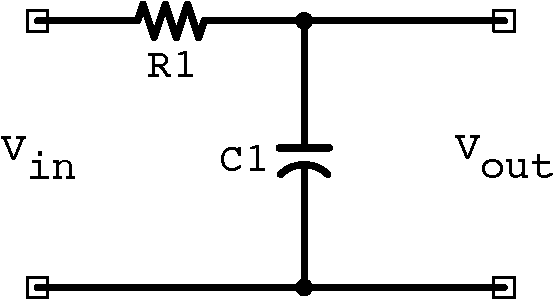
\includegraphics[resolution=300,scale=\diagramSize]{Introduktion/LowPassPassive}
	\caption{Et simpelt passivt filter}
	\label{fig:LowPassPassive}
\end{figure}
\noindent
%
Aktive filtre, som set på \autoref{fig:LowPassActive}, kræver tilført strøm, og benytter en operationsforstærker (OpAmp), sammen med modstande og kondensatorer. De kan håndtere meget lave frekvenser og kan øge spændingen på output, hvis ønsket. De er ofte nemmere at konstruere end passive filtre, og kan laves uden brug for store komponenter. De virker bedst ved frekvenser under 100kHz, som konsekvens af operationsforstærkerens båndbredde og slew-rate \parencite{BOOK:PracticalElectronicsforInventors} \fxnote{Hvad hedder slew rate på dansk?}.
%
\begin{figure}[H]
	\centering
	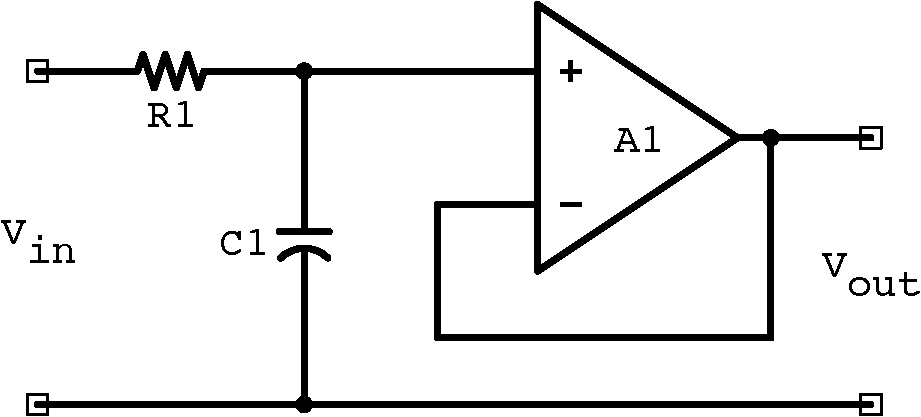
\includegraphics[resolution=300,scale=\diagramSize]{Figure/Introduktion/ActiveLowPass.pdf}
	\caption{Et simpelt aktivt filter, uden gain}
	\label{fig:LowPassActive}
\end{figure}
\noindent
%
Eftersom at mennekser kan høre lyde mellem ca. 20Hz og 20kHz \fxsource, er et aktivt filter at foretrække, da det er bedre egnet end passive filtre, i dette frekvensområde. Af samme årsag vil resten af denne rapport beskæftige sig med disse.
%
%
%
\section{Lavpasfiltre}
\label{Lavpasfiltre}
\begin{itemize}
  \item Knækfrekvenser
  \item Overførringsfunktionen
  \item Hældning 
  \item Formål 
  \item Illustrationer
  \item Formler
  \item Bode-plots?
  \item Brug afsnittet omkring hældningen i det lavfrekventeområde
\end{itemize}
Et lavpasfilter er et filter der, som navnet antyder, lader lave frekvenser passere igennem, men blokerer for høje. På \autoref{fig:LowPassActive} ses et aktivt lavpasfilter. At det er aktivt, betyder blot at der benyttes en operationsforstærker i sammenhæng med filtret.\\
Et lavpasfilter virker ved at kondensatoren, ved høje frekvenser, sænker sin impedans og således lader højre frekvenser gå til jord i stedet for at passere. Modstanden har stor impedans ved høje frekvenser, men lader lave frekvenser passere.\\
I opkoblingen fra \autoref{fig:LowPassActive} er der ingen forstærkning af inputsignalet, eftersom tilbagekoblingen går urørt fra $V_{out+}$ til operationsforstærkerens $V_{in-}$. En sådan tilbagekobling kan have fordele, selvom der ikke sker nogen forstærkning. Operationsforstærkerens høje inputimpedans forhindrer overdrevet belastning af filterets output og dens lave outputimpedans sørger for at filtrets afskæringsfrekvens ikke påvirkes af eventuelle ændringer af den efterfølgende impedans. Selvom filteret fra \autoref{fig:LowPassActive} ikke giver nogen spændingsforstærkelse over 1, giver det en meget høj effekt, grundet at inputimpedansen er langt højere end outputimpedansen. Med andre ord giver det god stabilitet til filteret. Et kredsløb med forstærkning, kan ses på \autoref{fig:LowPassActiveGain.pdfGain}.
%
\begin{figure}[H]
	\centering
	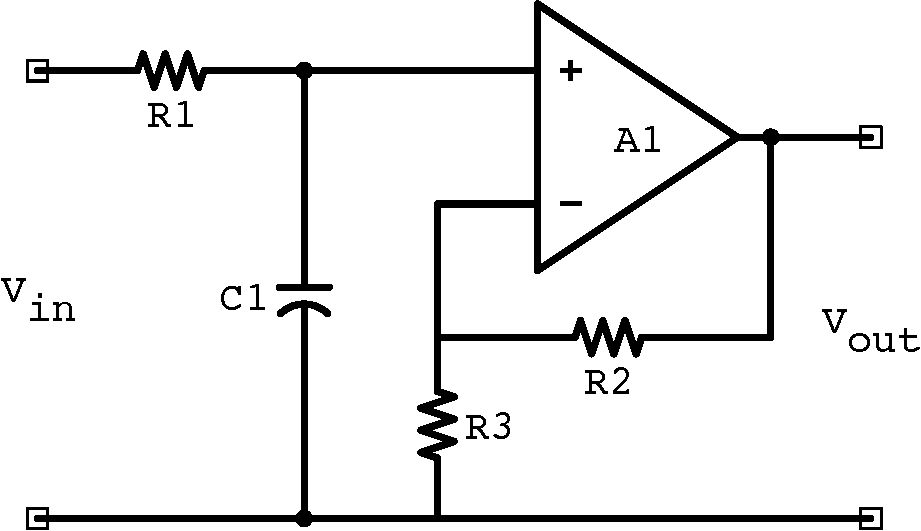
\includegraphics[resolution=300,scale=\diagramSize]{Figure/Introduktion/ActiveLowPassGain.pdf}
	\caption{Aktivt lavpasfilter med forstærkning}
	\label{fig:LowPassActiveGain}
\end{figure}
\noindent
\fxnote{Opdatér figur til ny stil}
%
%
%Forholdet mellem modstandene R1 og R2 dikterer $DC$-forstærkningen, og følger, for en ikke-inverterende operationsforstærker, formlen:
%%
%\begin{equation} \label{eq:LowPassDCGain}
%	DC_{gain}=\left(1+\frac{R_2}{R_1}\right)
%\end{equation}
%%
%Sammenholdt med filteret, følger den frekvensafhængige forstærkning af et lavpasfilter således formlen:
%%
%\begin{equation} \label{LowPassFqVGain}
%  V_{gain}=\frac{V_{out}}{V_{in}}=\frac{A_F}{\sqrt{1+\left(\frac{f}{f_c}\right)^2}}
%\end{equation}
%Hvor:\\
%$A_F$ = Forstærkningsfaktoren for operationsforstærkeren, $DC_{gain}$\\
%$f$ = Frekvensen af inputsignalet, i Hz\\
%$f_c$ = Afskæringsfrekvensen for filteret, i Hz\\
%Filteret har konstant forstærkning, $A_F$, fra 0Hz til lidt før afsksæringsfrekvensen $f_c$, hvorefter amplituden falder med en konstant rate på 20dB pr. dekade. Forløbet kan ses på \autoref{fig:FrequencyResponseCurve}.
%%
%\begin{figure}[H]
%	\centering
%	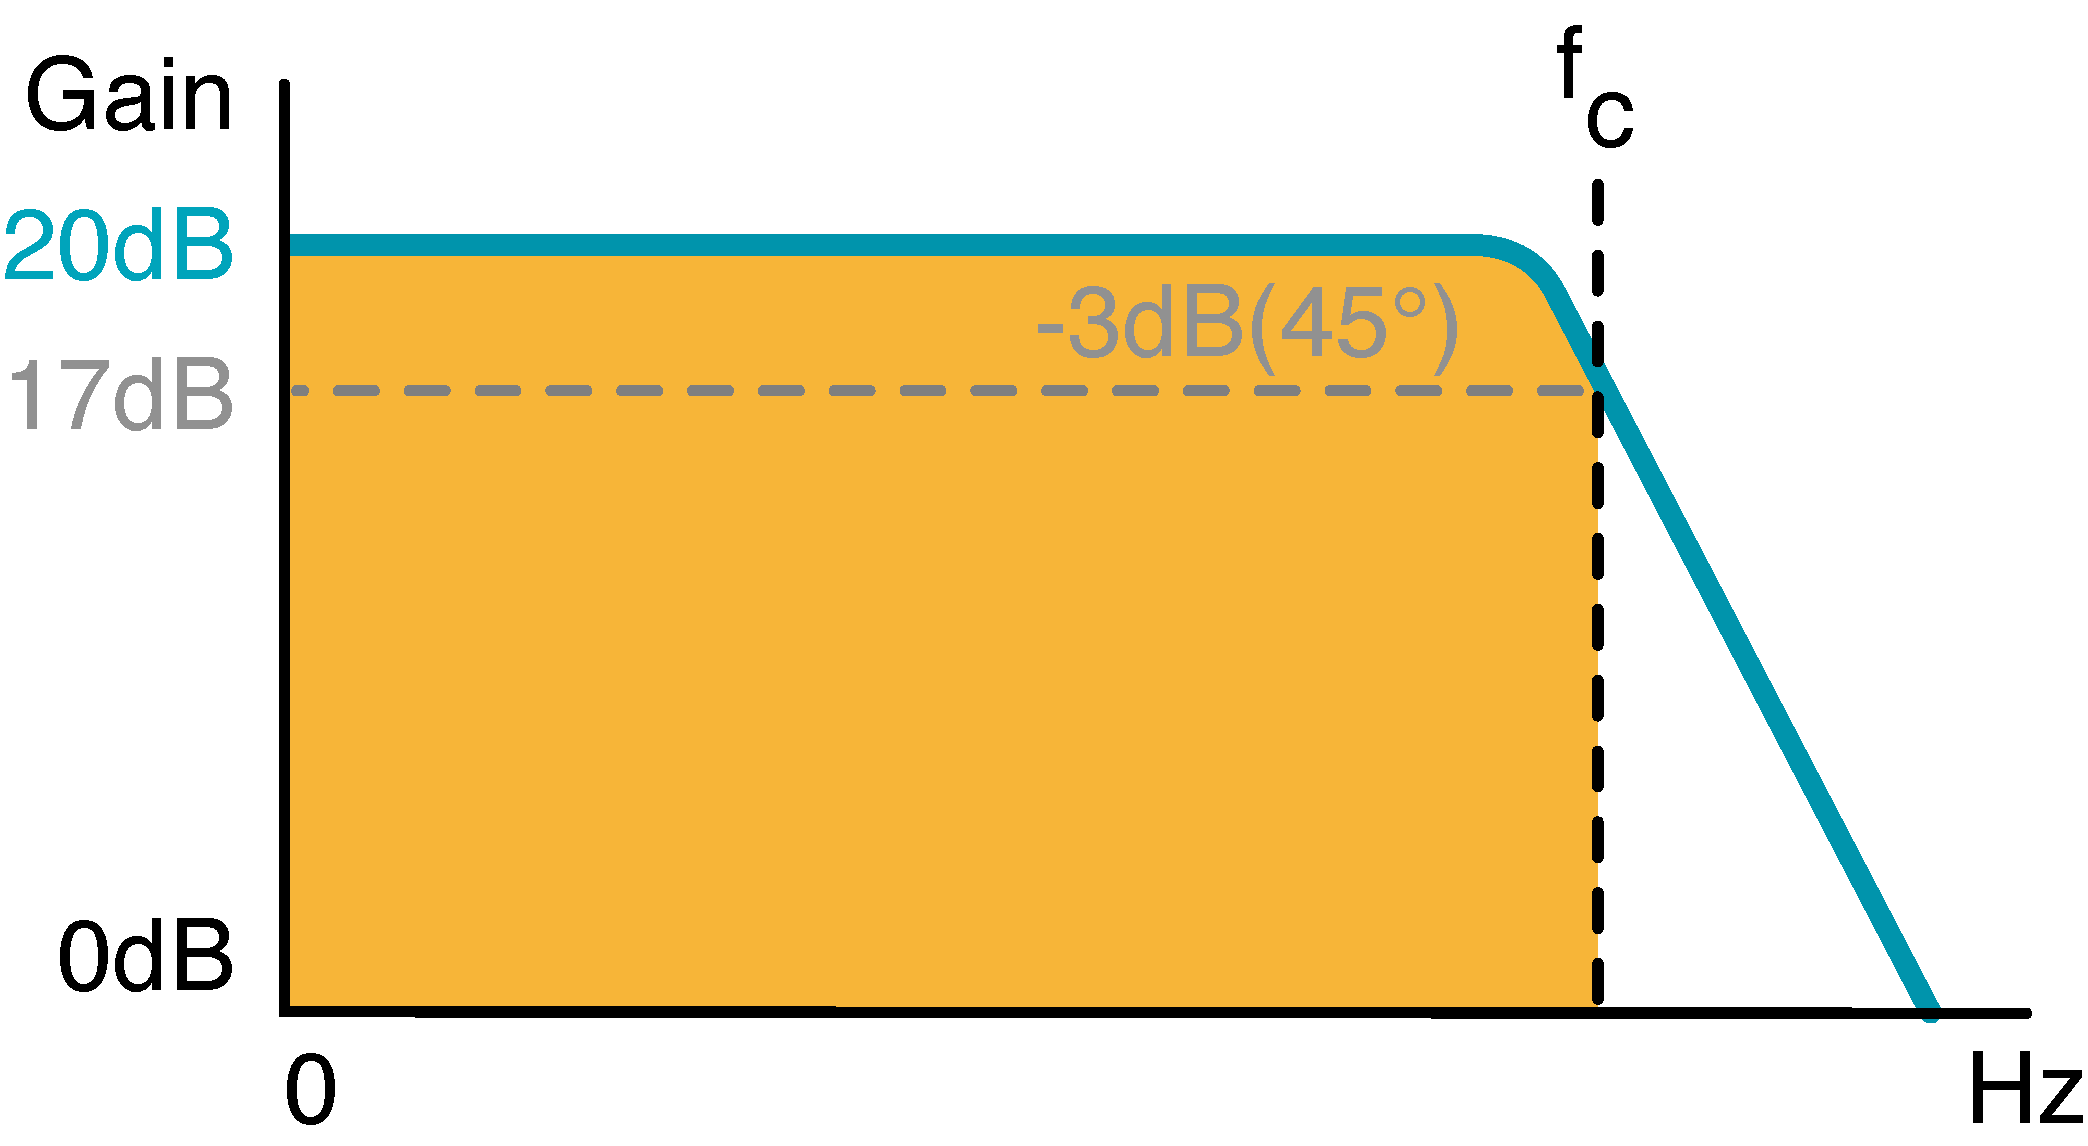
\includegraphics[resolution=300,width=\textwidth/2]{Introduktion/FrequencyResponseCurve}
%	\caption{Frekvensresponskurve for et lavpasfilter. Den orange del, er det frekvensområde som medtages i}
%	\label{fig:FrequencyResponseCurve}
%\end{figure}
%\noindent
%
%
%
\subsection{Fraktalordensfilter}
\label{Fraktalordensfilter}
%
\begin{itemize}
  \item Knækfrekvenser (fåes fra behandling af ISO)
  \item Hældning (fåes fra hældning i det lavfrekventeområde)
  \item Pinknoise filter? (hældning på 10dB/dec)
  \item Bode-plots
  \item Illustrationer
  \item Formler
  \item Hvorfor vi bruger fraktalordensfilter
\end{itemize}
\noindent
%
For at finde ud af hvilken orden vores filter skal være bruges formlen 
\begin{equation}
	a=20*log(10^x)
\end{equation}

%
\subsubsection{Hældning i det lavfrekventeområde}
\label{HaeldningIDetLavfrekventeområde}
%
\begin{itemize}
	\item Bruges til at bestemme hældningen på lavpas-filtrene.
	\item Vi vil gerne lave et filter, som kan sættes efter hinanden for at få en større hældning så derfor runder vi op til hele 5'ere, da den afrundning vil være uhørbar
\end{itemize}

I \autoref{tab:ISO226Difference630Hz} forefindes det nye datasæt i frekvensområdet fra 20Hz til 630Hz, hvor de resterende datapunkter forefindes i \autoref{app:ISO226Difference}. 
%
\begin{table}[H]
\centering
\resizebox{\textwidth}{!}{%
\begin{tabular}{|r|r|r|r|r|r|r|r|r|}
\hline
\multicolumn{1}{|l|}{Frekvens{[}Hz{]}} & \multicolumn{1}{l|}{20phon} & \multicolumn{1}{l|}{30phon} & \multicolumn{1}{l|}{40phon} & \multicolumn{1}{l|}{50phon} & \multicolumn{1}{l|}{60phon} & \multicolumn{1}{l|}{70phon} & \multicolumn{1}{l|}{80 phon} & \multicolumn{1}{l|}{90phon} \\ \hline
20 & 30.6 & 25.8 & 20.9 & 15.7 & 10.5 & 5.3 & 0 & -5.3 \\ \hline
25 & 28.5 & 24.3 & 19.7 & 14.9 & 10 & 5 & 0 & -5 \\ \hline
31.5 & 26.4 & 22.8 & 18.6 & 14.1 & 9.5 & 4.8 & 0 & -4.7 \\ \hline
40 & 24.6 & 21.2 & 17.3 & 13.2 & 8.9 & 4.5 & 0 & -4.4 \\ \hline
50 & 22.3 & 19.6 & 16.1 & 12.3 & 8.3 & 4.2 & 0 & -4.2 \\ \hline
63 & 20.2 & 17.8 & 14.7 & 11.2 & 7.5 & 3.8 & 0 & -3.9 \\ \hline
80 & 18 & 16 & 13.3 & 10.2 & 6.9 & 3.4 & 0 & -3.5 \\ \hline
100 & 15.9 & 14.3 & 11.9 & 9.1 & 6.2 & 3.1 & 0 & -3.2 \\ \hline
125 & 13.8 & 12.5 & 10.5 & 8.1 & 5.5 & 2.8 & 0 & -2.8 \\ \hline
160 & 11.6 & 10.6 & 8.9 & 6.9 & 4.7 & 2.4 & 0 & -2.4 \\ \hline
200 & 9.6 & 8.9 & 7.5 & 5.8 & 4 & 2 & 0 & -2 \\ \hline
250 & 7.7 & 7.2 & 6.1 & 4.7 & 3.2 & 1.6 & 0 & -1.7 \\ \hline
315 & 5.8 & 5.5 & 4.7 & 3.6 & 2.5 & 1.3 & 0 & -1.3 \\ \hline
400 & 4 & 3.8 & 3.3 & 2.6 & 1.8 & 0.9 & 0 & -0.9 \\ \hline
500 & 2.5 & 2.5 & 2.2 & 1.7 & 1.2 & 0.6 & 0 & -0.7 \\ \hline
630 & 1.3 & 1.3 & 1.1 & 0.9 & 0.6 & 0.3 & 0 & -0.4 \\ \hline
\end{tabular}%
}
\caption{Det nye datasæt, som består af differencerne mellem referencen og de specifikke phon-kurver, samt lydtryksniveauerne målt ved hver frekvens. Datasættet fokuserer kun på frekvensområdet 20Hz til 630Hz.}
\label{tab:ISO226Difference630Hz}
\end{table}
%


\begin{table}[H]
\centering
\resizebox{\textwidth}{!}{%
\begin{tabular}{|r|r|r|r|r|r|r|r|r|}
\hline
\multicolumn{1}{|l|}{Frekvens{[}Hz{]}} & \multicolumn{1}{l|}{20phon} & \multicolumn{1}{l|}{30phon} & \multicolumn{1}{l|}{40phon} & \multicolumn{1}{l|}{50phon} & \multicolumn{1}{l|}{60phon} & \multicolumn{1}{l|}{70phon} & \multicolumn{1}{l|}{80 phon} & \multicolumn{1}{l|}{90phon} \\ \hline
20-630 & 29.3 & 24.5 & 19.8 & 14.8 & 9.9 & 5 & 0 & 0 \\ \hline
\end{tabular}%
}
\caption{Hældningen mellem 20Hz og 630Hz for hver phon-kurve, udregnet ved differencen derimellem.}
\label{tab:HaeldningFra20til630}
\end{table}
\noindent
%
Brugt til at finde stepsize på vores filter, så når der er en ændring i volumen på 5dB skal vi skifte filter. 

\begin{table}[H]
\centering
\resizebox{\textwidth}{!}{%
\begin{tabular}{|r|r|r|r|r|r|r|r|r|}
\hline
\multicolumn{1}{|l|}{Frekvens{[}Hz{]}} & \multicolumn{1}{l|}{20phon} & \multicolumn{1}{l|}{30phon} & \multicolumn{1}{l|}{40phon} & \multicolumn{1}{l|}{50phon} & \multicolumn{1}{l|}{60phon} & \multicolumn{1}{l|}{70phon} & \multicolumn{1}{l|}{80 phon} & \multicolumn{1}{l|}{90phon} \\ \hline
20-200 & 21 & 16.9 & 13.4 & 9.9 & 6.5 & 3.3 & 0 & -3.3 \\ \hline
200-630 & 8.3 & 7.6 & 6.4 &4.9 & 3.4 & 1.7 & 0 & -1.6\\ \hline
200-2000 & 12 & 10.7 & 8.9 & 6.8 & 4.6 & 2.3 & 0 & -2.3\\ \hline
\end{tabular}%
}
\caption{Hældningen per dekade, udregnet ved differencen derimellem.}
\label{tab:HaeldningFra20til630}
\end{table}
\noindent
%
Bruges til at finde den hældning vores filter skal have. De tal der står der skal halveres fordi de er regnet med en stepsize på 10dB, så ved 70phon (mellem 20 og 200) skal 3.3 dB være 1.7 dB (1.65)?. Hældningen ville være 3.3 dB per 2 dekader. 

\section{Operationsforstærker}
\label{OpAmp}
%
\begin{itemize}
  \item Ideelle og reelle operationsforstærkere
  \item Inverterende og ikke-inverterende 
  \item Illustrationer
  \item Formler
  \item Tilbagekobling - hvorfor er det godt? 
  \item Beta-værdier og udregninger 
\end{itemize}

\section{Dimensionering af fraktalordens lavpasfilter}
\label{DimensioneringAfFraktalordensLavpasfilter}
%
\begin{itemize}
  \item Signalet vej igennem vores filter
  \item Komponent valg og værdier (modstande, kondensatorer, operationsforstærker mm.) 
  \item Beregninger af komponent værdier
  \item Illustrationer og simulationer
\end{itemize}





%\section{Delefiltre}
\label{Delefiltre}
Som vist i \fxnote{Hvor er det beskrevet? i Saras ISO-databehandling}, er der tre nævneværdige segmenter på kurven. Hvert segment skal behandles forskelligt, hvorfor der er behov for først at dele signalet ind i tre delsignaler; et fra 0-1000hz, et fra 1000-8000hz og et fra 8000hz og opefter. Ifølge \textcite{PDF:Elektroakustik}, ligger frekvenslejet for grundtonen for et typisk musikinstrument mellem  40Hz og 1000Hz, med overtonefrekvenser langt over den menneskelige hørelse. Dertil kommer de lyde som kan produceres fra en computer eller synthesizer.\\\textcite{STD:ISO226} Afdækker kun den menneskelige hørelse inden for frekvenslejet 20Hz to 12500Hz, men frekvenserne fra 20Hz og nedefter og fra 12kHz og opefter kan med fordel medtages i henholdavis et lav- og højpass filter, da det udgør et simplere filter, og samtidig undgår uforudsete konsekvenser for lyden ved fraskæring, omend, i nogle tilfælde, uden for det hørbare område.\\
Et analogt delefilter bør i teorien kunne have et uendeligt antal band-pass filtre, men er begrænset af hvor præcist et udsnit der kan laves. Man kan eksempelvis ikke lave et filter som udelukkende lukker 1kHz-toner igennem, fordi der er en unøjagtighed nær cutoff-frekvensen, som kaldes for et overgangsbånd, som kan ses på \autoref{fig:OvergangsbaandIllustration}.
%
\begin{figure}[H]
	\centering
	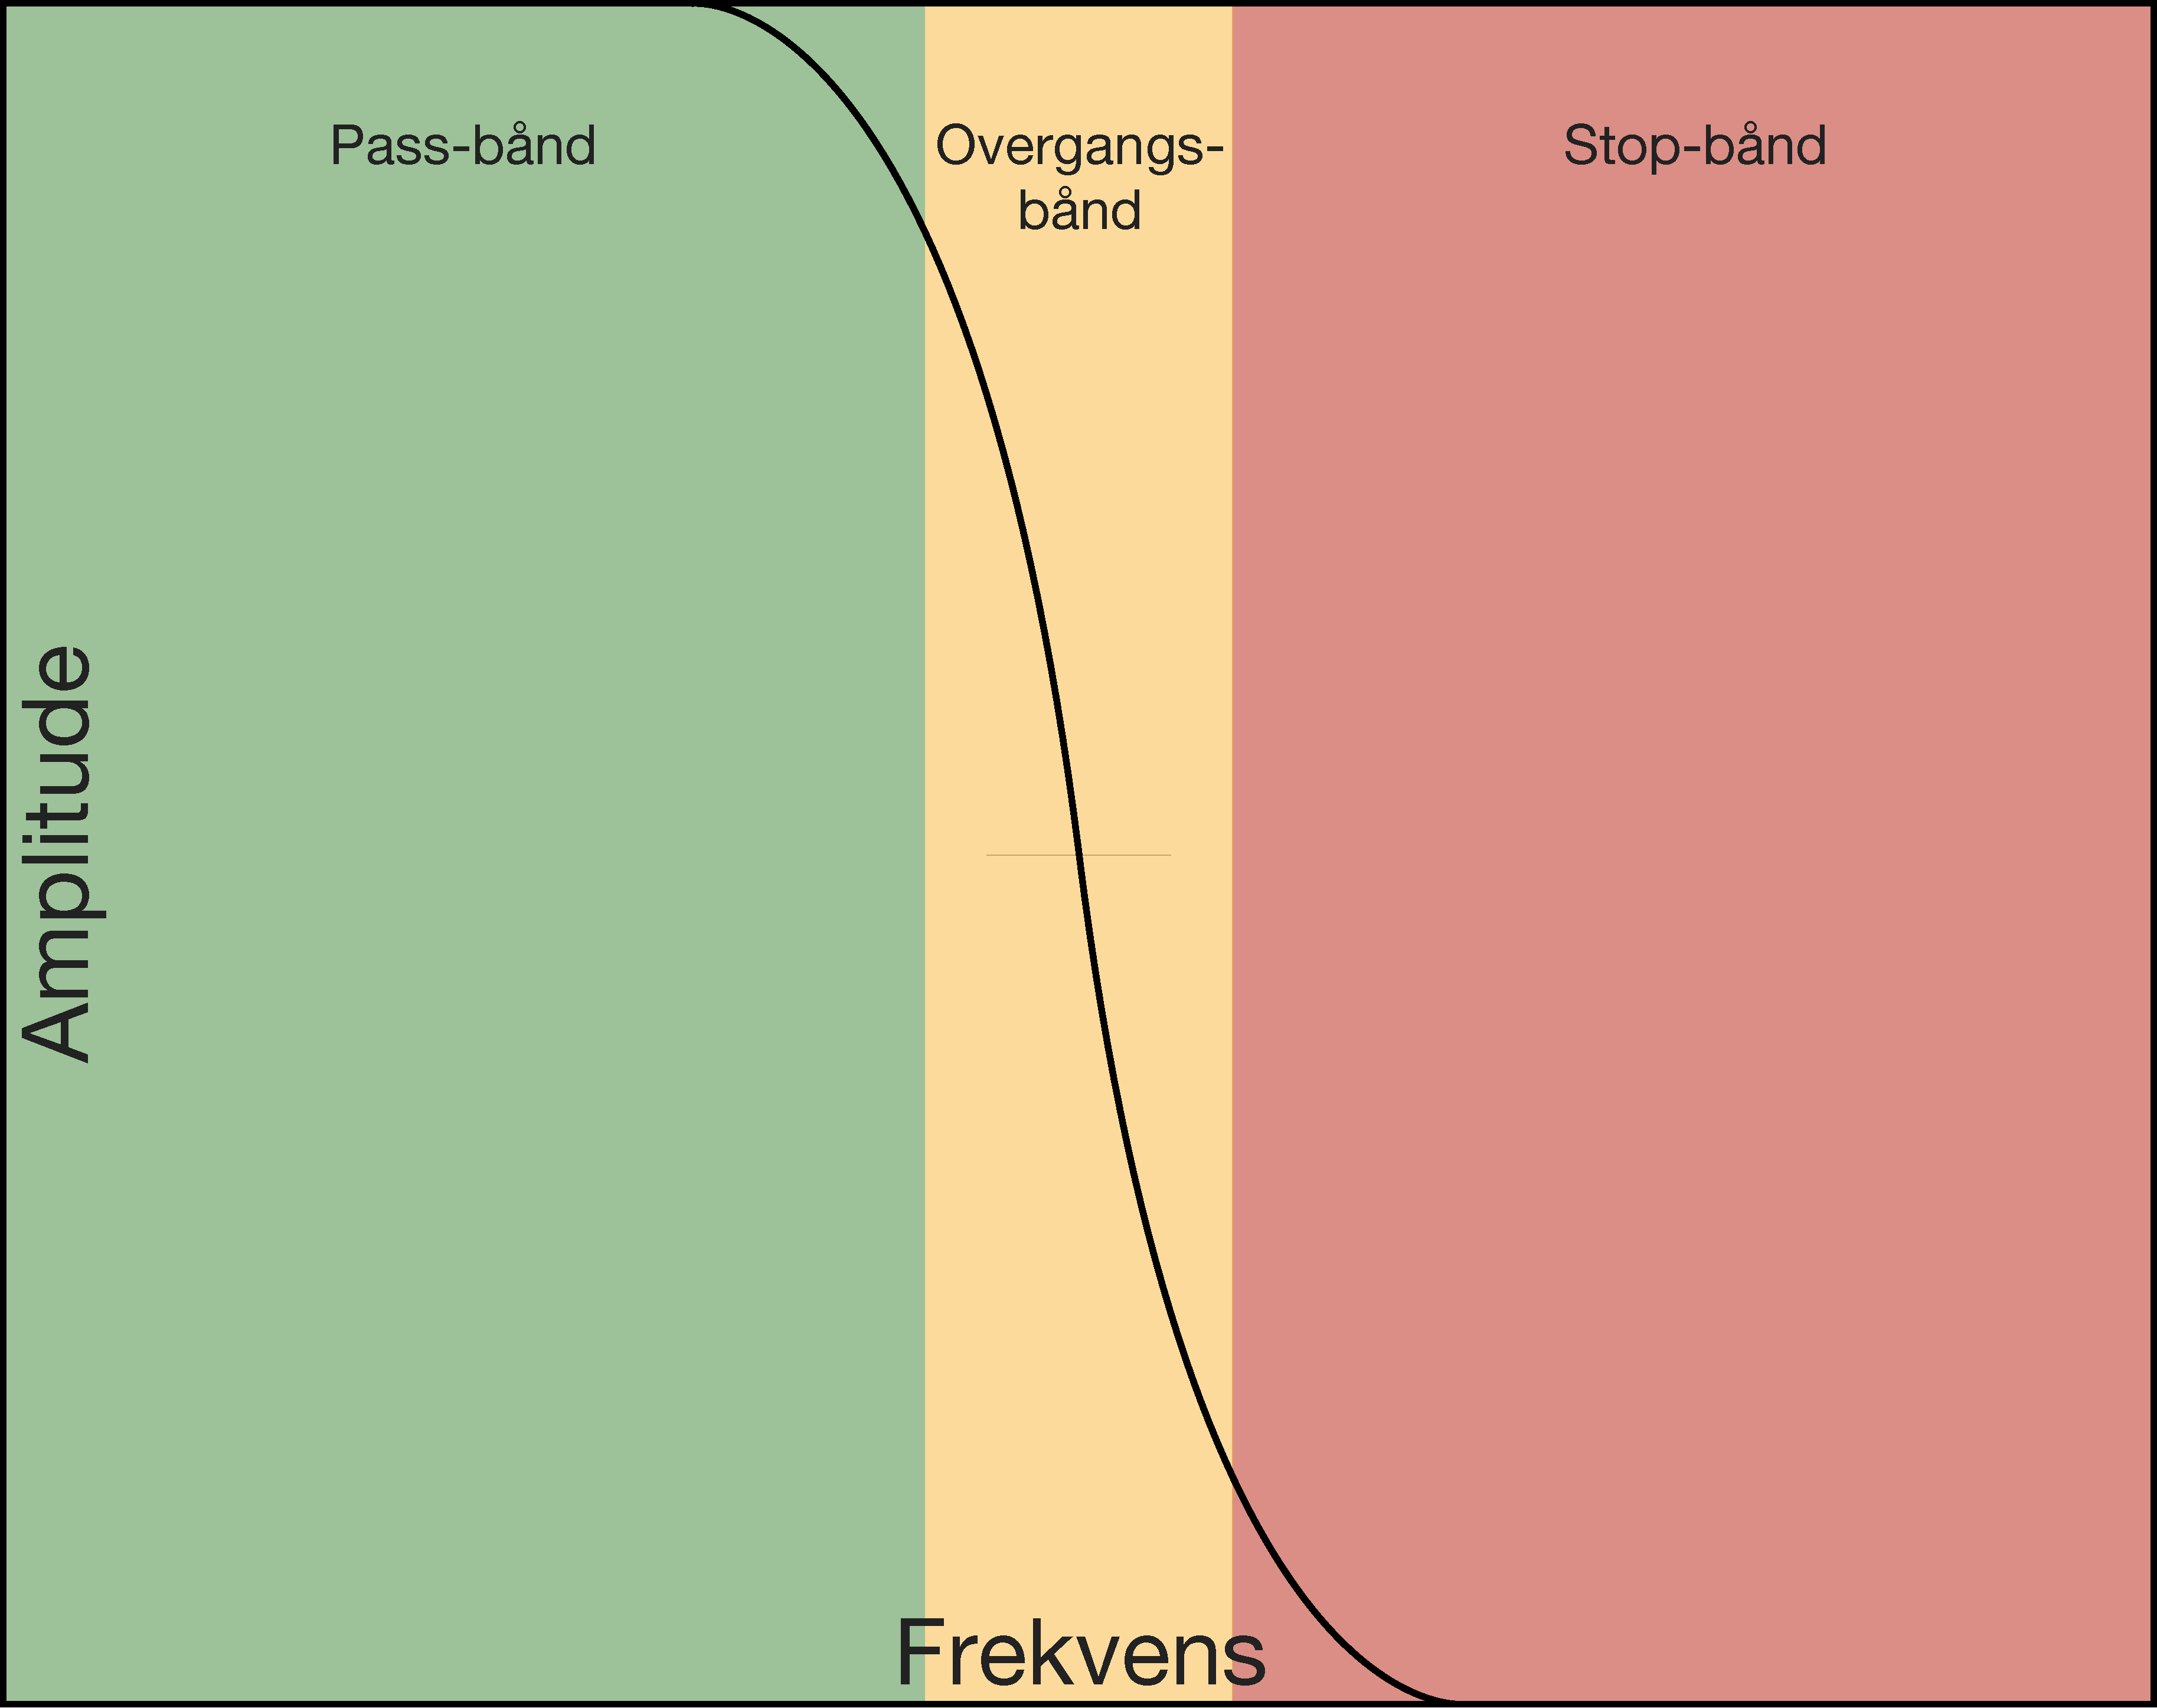
\includegraphics[resolution=300,width=\textwidth/2]{Introduktion/OvergangsbaandIllustration}	
	\caption{Illustration af et typisk overgangsbånd for et low-pass filter. Den grønne firkant er hvad et ideelt filter ville lade passere, men i virkeligheden er det alt under kurven, som medtages. Den gule firkant er således overgangsbåndet, altså et biprodukt af filtret,}
	\label{fig:OvergangsbaandIllustration}
\end{figure}
\noindent
%
Overgangsbåndet er en bivirkning ved alle analoge filtre, men kan minimeres ved at øge ordenen af filteret. Det har dog andre ulemper, som vil blive diskuteret senere.\\
%
%
%
\subsection{Aktive- og passive filtre}
\label{Aktive- og passive filtre}
Filtre kan være enten passive eller aktive, hver med sine egenskaber. Hvilken filtertype man vælger, afhænger af hvilke egenskaber man ønsker, såvel som krav til pris og fysisk størrelse.\\
Passive filtre har den fordel at de kan operere uden tilført strøm, som navnet angiver. De benytter kun passive komponenter som modstande, kondensatorer og spoler og virker bedst ved frekvenser mellem 100Hz og 300MHz \parencite{BOOK:PracticalElectronicsforInventors}. Dets lavere frekvensområde, dets større kapacitans og induktans, hvilket kræver fysisk større komponenter, deraf den nedre grænse. Ved høje frekvenser vil komponenterne interferere med hinanden, deraf den øvre grænse.\\
Aktive filtre, modsat passive, kræver tilført strøm, og benytter en operationsforstærker (OpAmp), sammen med modstande og kondensatorer. De kan håndtere meget lave frekvenser og kan øge spændingen på output, hvis ønsket. De er ofte nemmere at konstruere end passive filtre, og kan laves uden brug for store komponenter. De virker bedst ved frekvenser under 100kHz, som konsekvens af operationsforstærkerens båndbredde og slew-rate \fxnote{Hvad hedder slew rate på dansk?}.\\
Eftersom at mennekser kan høre lyde mellem ca. 20Hz og 20kHz, er et aktivt delefilter at foretrække, da det er bedre egnet end passive filtre, i dette frekvensområde. Af samme årsag vil resten af denne rapport beskæftige sig med disse.
%
%
%
\subsection{Lavpasfiltre}
\label{Lavpasfiltre}
Et lavpasfilter er et filter der, som navnet antyder, lader lave frekvenser passere igennem, men blokerer for høje. På \autoref{fig:ActiveLowPass} ses et aktivt lavpasfilter. At det er aktivt, betyder blot at der er tilkoblet en operationsforstærker efter filtret.
%
\begin{figure}[H]
	\centering
	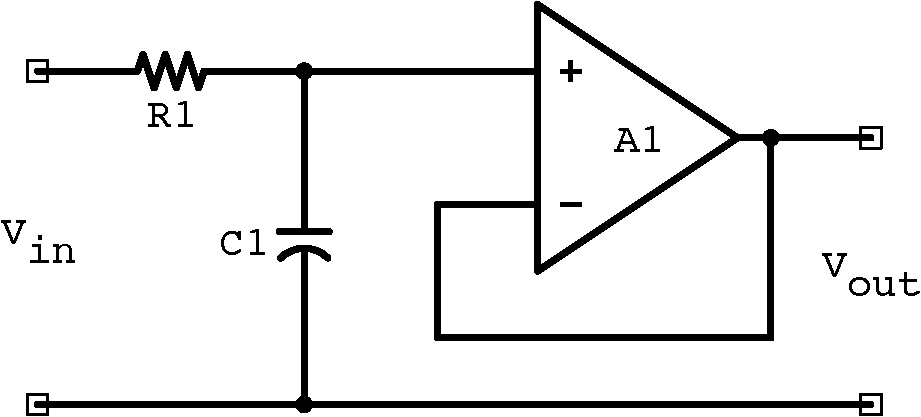
\includegraphics[resolution=300,scale=0.5]{Figure/Introduktion/ActiveLowPass.pdf}
	\caption{Aktivt Lavpasfilter}
	\label{fig:ActiveLowPass}
\end{figure}
\noindent
%
Et lavpasfilter virker ved at kondensatoren, ved høje frekvenser, sænker sin impedans og således lader højre frekvenser gå til jord i stedet for at passere. Modstanden har stor impedans ved høje frekvenser, men lader lave frekvenser passere. Formlen for $V_{out}$ for et passivt filter er:
%
\begin{equation} \label{eq:LowPass_Vout}
	V_{out}=\frac{Z_c}{Z_c+R}*V_{in}
\end{equation}
%
Men det som er mest interessant inden for elektronik, er er \textit{forholdet} mellem $V_{out}$ og $V_{in}$, som kan udtrykkes således:
\begin{equation} \label{eq:LowPass_VOutVin}
	 \left\lvert\frac{V_{out}}{V_{in}}\right\rvert=\frac{1}{\sqrt{1+(\omega RC)^2}}
\end{equation}
\fxnote{Forklar hvad de forskellige ting er i formlerne}
%
Et aktivt filter er blot et passivt filter efterfulgt af en operationsforstærker. I opkoblingen fra \autoref{fig:ActiveLowPass} er der ingen forstærkning af inputsignalet, eftersom tilbagekoblingen går urørt fra $V_{out+}$ til operationsforstærkerens $V_{in-}$. En sådan tilbagekobling kan have fordele, selvom der ikke sker nogen forstærkning. Operationsforstærkerens høje inputimpedans forhindrer overdrevet belastning af filterets output og dens lave outputimpedans sørger for at filtrets afskæringsfrekvens ikke påvirkes af eventuelle ændringer af den efterfølgende impedans. Selvom filteret fra \autoref{fig:Aktivt Lavpasfilter} ikke giver nogen spændingsforstærkelse over 1, giver det en meget høj effekt, grundet at inputimpedansen er langt højere end outputimpedansen. Med andre ord giver det god stabilitet til filteret, men giver ikke nogen spændingsforstærkning. Et kredsløb med forstærkning, kan ses på \autoref{fig:ActiveLowPassGain}.
%
\begin{figure}[H]
	\centering
	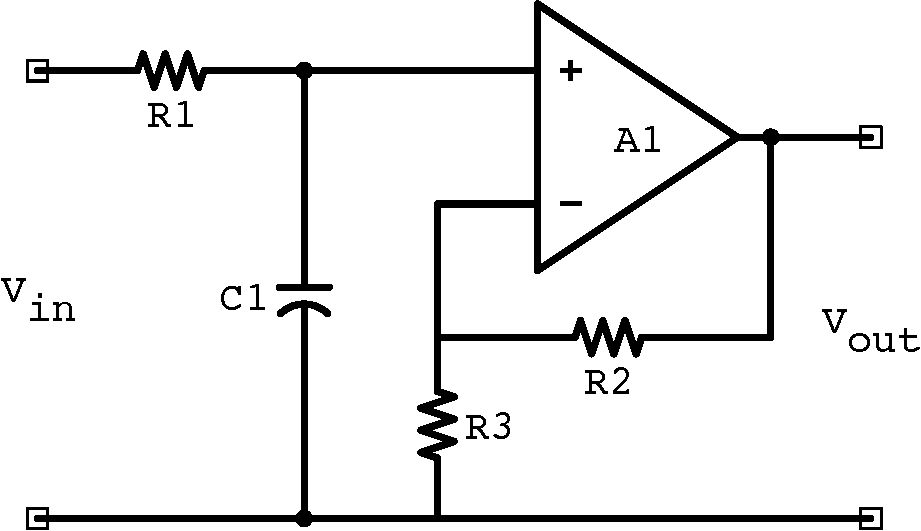
\includegraphics[resolution=300,scale=0.5]{Figure/Introduktion/ActiveLowPassGain.pdf}
	\caption{Aktivt lavpasfilter med forstærkning}
	\label{fig:ActiveLowPassGain}
\end{figure}
\noindent
%
Forholdet mellem modstandene R1 og R2 dikterer $DC$-forstærkningen, og følger, for en ikke-inverterende operationsforstærker, formlen:
%
\begin{equation} \label{eq:LowPassDCGain}
	DC_{gain}=\left(1+\frac{R_2}{R_1}\right)
\end{equation}
%
Sammenholdt med filteret, følger den frekvensafhængige forstærkning af et lavpasfilter således formlen:
%
\begin{equation} \label{LowPassFqVGain}
  V_{gain}=\frac{V_{out}}{V_{in}}=\frac{A_F}{\sqrt{1+\left(\frac{f}{f_c}\right)^2}}
\end{equation}
Hvor:\\
$A_F$ = Forstærkningsfaktoren for operationsforstærkeren, $DC_{gain}$\\
$f$ = Frekvensen af inputsignalet, i Hz\\
$f_c$ = Afskæringsfrekvensen for filteret, i Hz\\
Filteret har konstant forstærkning, $A_F$, fra 0Hz til lidt før afsksæringsfrekvensen $f_c$, hvorefter amplituden falder med en konstant rate på 20dB pr. dekade. Forløbet kan ses på \autoref{fig:FrequencyResponseCurve}.
%
\begin{figure}[H]
	\centering
	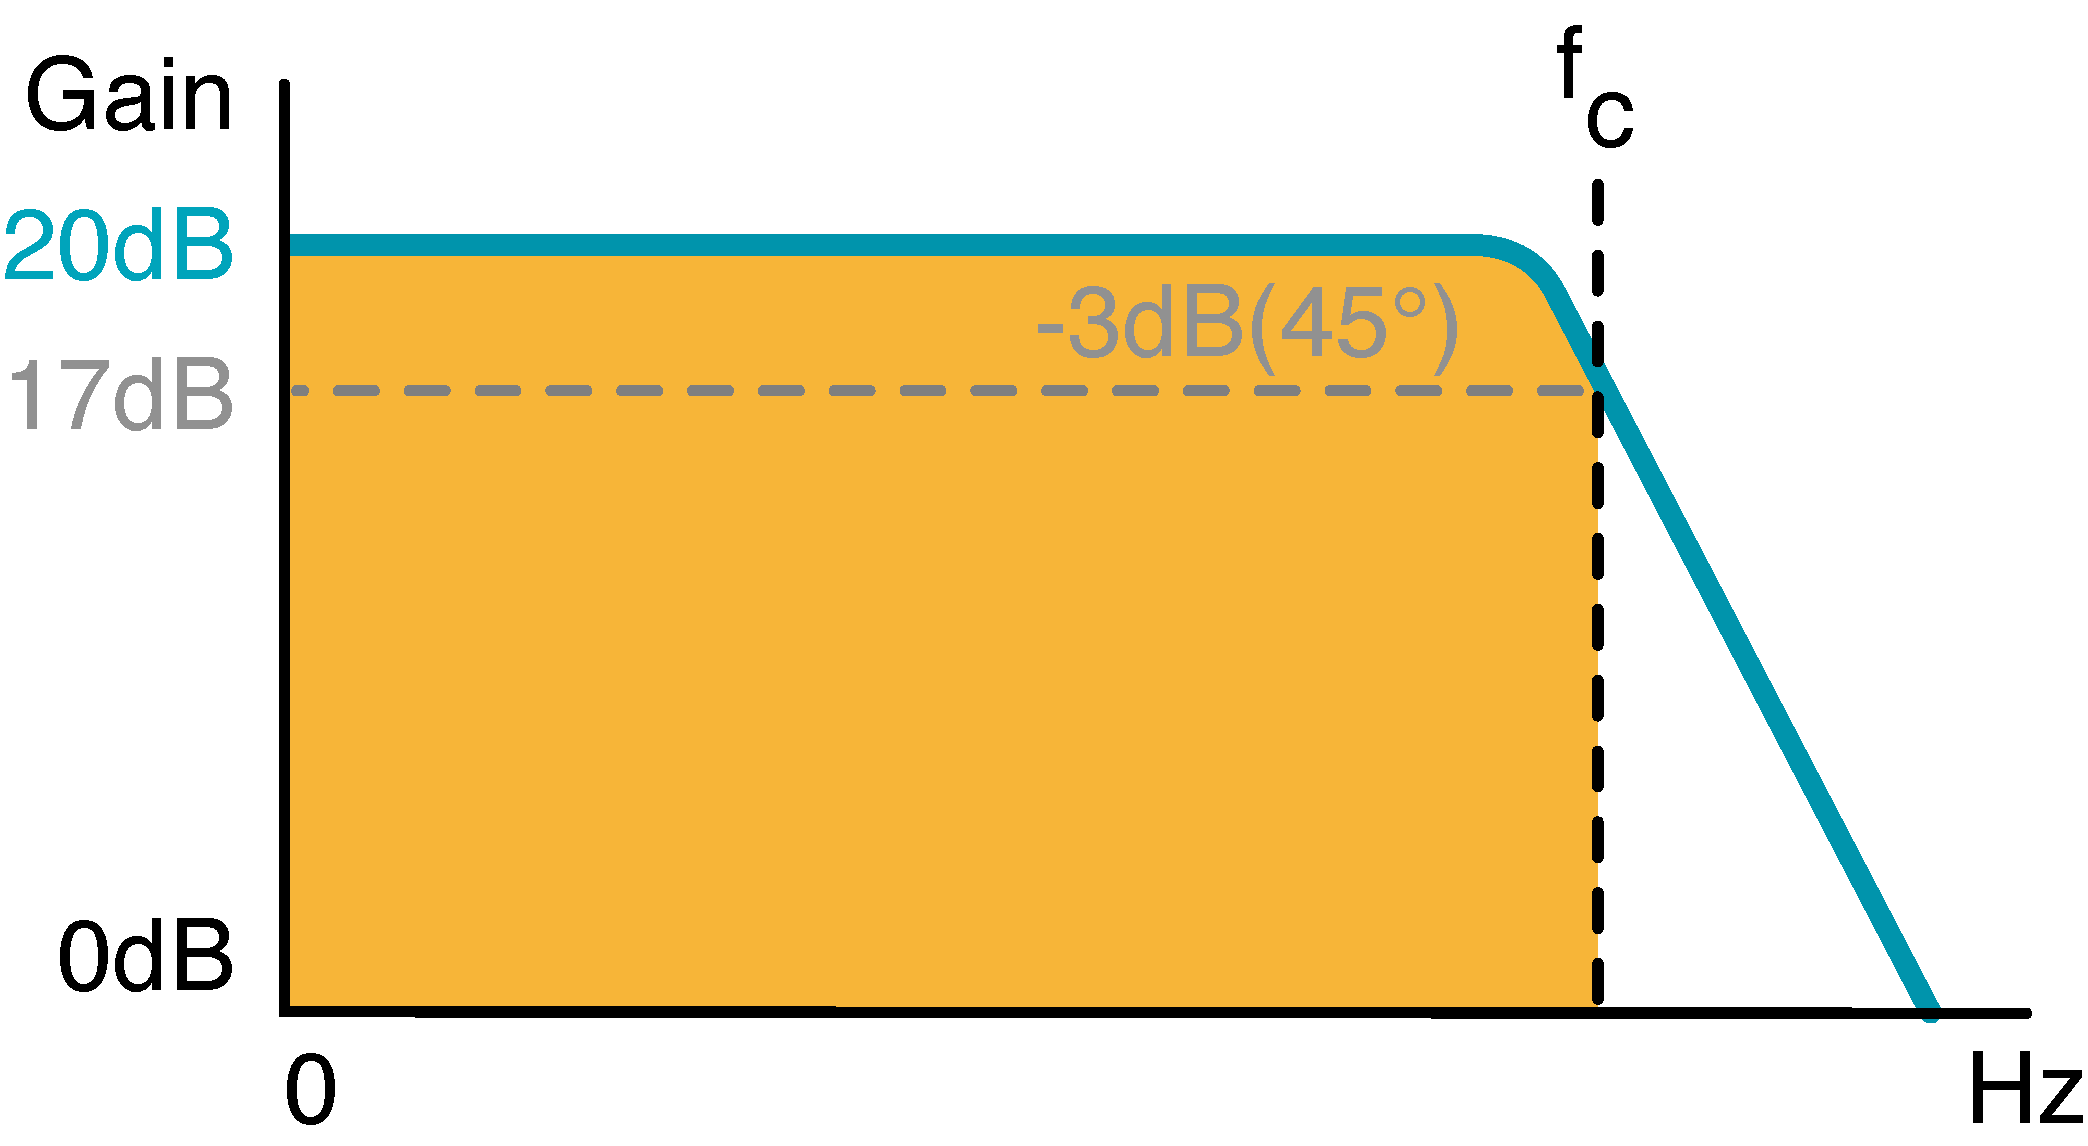
\includegraphics[resolution=300,width=\textwidth/2]{Introduktion/FrequencyResponseCurve}
	\caption{Frekvensresponskurve for et lavpasfilter. Den orange del, er det frekvensområde som medtages i}
	\label{fig:FrequencyResponseCurve}
\end{figure}
\noindent
X\fxnote{skriv figurtekst}
%
%
%
\subsection{Højpasfiltre}
\label{Hoejpasfiltre}
Et højpasfilter er det modsatte af et lavpasfilter, forstået på den måde at det kun lader høje frekvenser passere. Et aktivt lavpasfilter kan ses på....
%
%
%
\subsection{Båndpasfiltre}
\label{Baandpasfiltre}

%Et 
%
%For at lave et delefilter med tre frekvensbånd sammensættes blot et low-pass, band-pass og high-pass filter.
%

%\section{Signalsplejsning} 
\label{Signalsplejsning} 
En opamp forstærker forskellen mellem to spændinger. Det betyder at spændingsforskellen mellem inputterminalerne V+ og V- forstærkes. En ideel opamp kan forstærke en spændingsforskel uendeligt, hvilket medfører at selv en lille spændingsforskel mellem V+ og V- forstærkes uendeligt meget.    
Den ideelle op amp eksisterer kun i teorien, da det antages at kredsløbet er bygget af ideelle komponenter med ideelle egenskaber.
%
\begin{figure}[H]
\centering
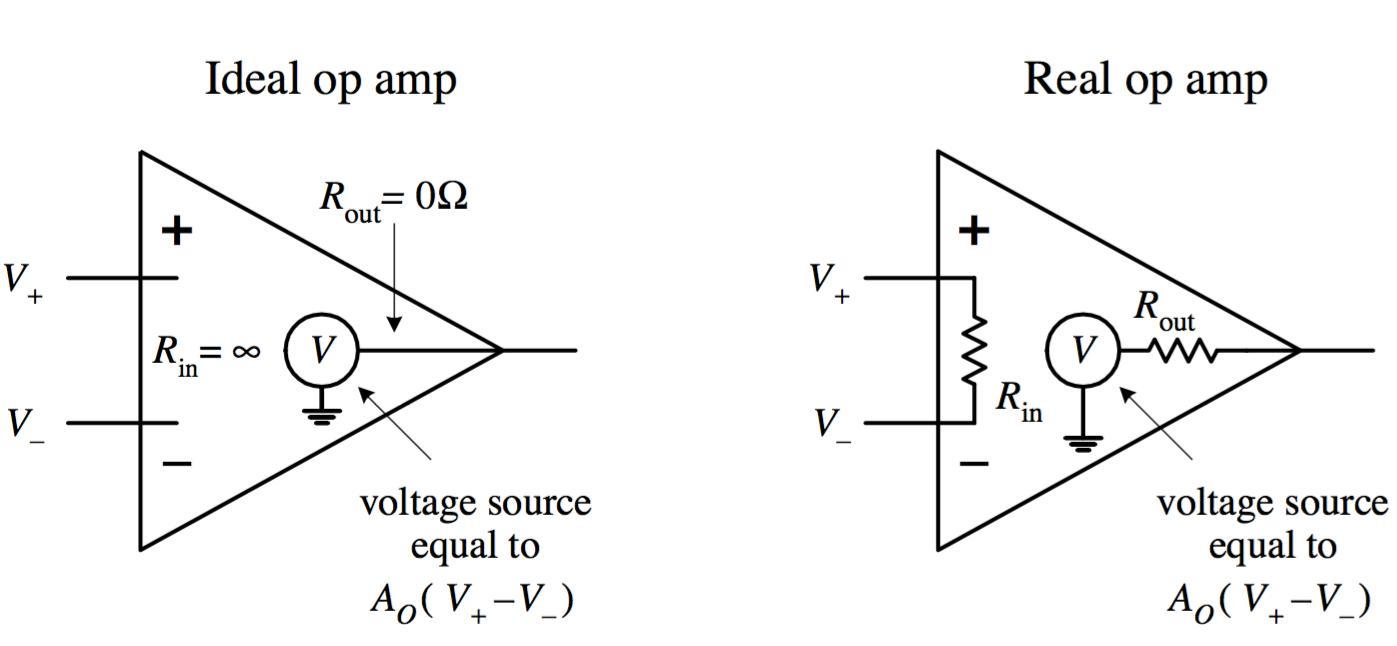
\includegraphics[resolution=300,width=\textwidth]{Figure/Introduktion/IdealRealOpAmp.png}
\caption{manglende figurtekst}
\label{fig:IdealRealOpAmp}
\end{figure}
\noindent
%
Egenskaberne ved en op amp kan siges at være ideelle fordi forstærkningen (Ao) er uendelig, udgangsimpedansen (ZOUT) er 0, indgangsimpedansen (ZIN) er uendelig og der ingen strøm løber mellem V+ og V-. I praksis er det ikke mulig at bygge et sådant kredsløb. En reel op amp har typisk egenskaber der gør den i stand til at forstærke mellem 100.000 og 1.000.000 gange, have en udgangsimpedans mellem 10 og 1K Ohm, en indgangsimpedans mellem 1M ohm og 1T Ohm og en strøm løbende mellem V+ og V- på få nanoampere eller picoampere.\\
%
Alligevel kan det være hensigtsmæssigt at betragte en reel op amp som om den var ideel,  da generaliseringen ikke skaber nogen nævneværdi fejl, men blot gøre det lettere at beregne på kredsløb hvori den indgår.\\
%
Udgangssignalet (VOUT) fra en op amp afhænger af indgangssignalet (VIN=(V+-V-)) og forstærkningen (Ao). Dette kan udtrykkes som VOUT = Ao(V+-V-). Forstærkningen kan derfor udtrykkes som Ao=VOUT/(V+-V-).    
%
\begin{figure}[H]
\centering
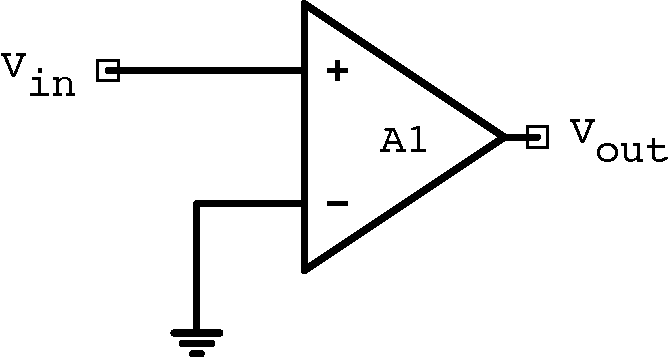
\includegraphics[resolution=300,width=\textwidth/2]{Figure/Introduktion/NonInvertingOpAmp.pdf}
\caption{manglende figurtekst}
\label{fig:IkkeInverterendeOpAmp}
\end{figure}
\noindent
%
I eksemplet ovenfor er den inverterende indgang V- forbundet til 0V og den ikkeinverterende indgang V+ forbundet til VIN. VOUT kan derfor udtrykkes ved at indsætte argumentet for V+ og V- i formlen VOUT = Ao(V+-V-) hvilket giver anledning til omskrivningen VOUT = Ao(VIN-0V) = AoVIN. Forstærkningen kan derfor udtrykkes som Ao=VOUT/VIN. Ideelt set forstærkes VIN uendeligt, hvilket betyder at VOUT er uendelig stor og bærer samme fortegn som VIN.
%
\begin{figure}[H]
\centering
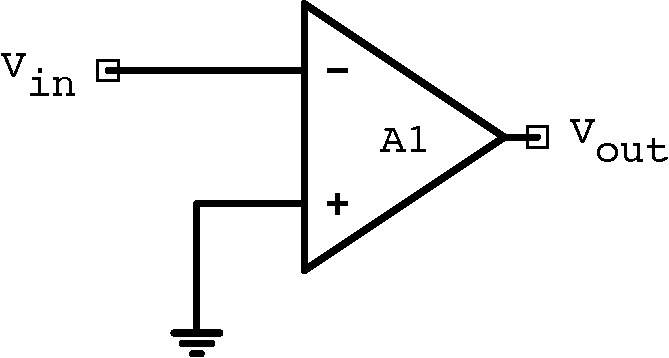
\includegraphics[resolution=300,width=\textwidth/2]{Figure/Introduktion/InvertingOpAmp.pdf}
\caption{manglende figurtekst}
\label{fig:InverterendeOpAmp}
\end{figure}
\noindent
%
I eksemplet ovenfor er det i stedet den ikkeinverterende indgang V+ som forbindes til 0V og den inverterende indgang V- som forbindes til VIN. VOUT kan igen udtrykkes ved at indsætte argumentet for V+ og V- i formlen VOUT = Ao(V+-V-) hvilket giver anledning til omskrivningen VOUT = Ao(0V-VIN) = -AoVIN. Forstærkningen kan derfor udtrykkes som -Ao=VOUT/VIN. Ideelt set forstærkes VIN minus uendeligt, hvilket betyder at VOUT er uendelig stor og bærer modsatte fortegn som VIN.\\
%
En Op amp kan altså ved en simpel kobling hvor et indgangssignal føres til den inverterende indgang og den ikkeinverterende indgang til ground, som vist ovenfor, ideelt inverterer og forstærker indgangssignalsignalet uendeligt. Reelt er det ikke muligt at forstærke signalet uendeligt selvom den ideelle opamp tillader det. Denne uoverenstemmelse ses der dog bort fra da det sjældent er intensionen at forstærke et  signal uendeligt, men derimod at forstærke med en endelig skaleringfaktor, hvorved problemet viser sig at være ubetydende.\\
%
Forstærkningen kan eksempelvis styres ved at koble en opamp så der indgår det der hedder et negativt feedback. Negativt feedback betyder at hele eller dele af udgangssignalet (VOUT) sendes tilbage til den inverterende indgang (V-). V- kan i udtrykket VOUT = Ao(V+-V-) omskrives til at udtrykke den spændning som sendes tilbage via feedback koblingen. Dette gøres ved at indsætte fVOUT på V- plads i udtrykket VOUT = Ao(V+-fVOUT). fVOUT  kan ikke overstige VOUT, men feedbackkoblingen kan ske via en resistor eller en capacitor hvorved det kun er en brøkdel af signalet som sendes tilbage som feedback. Udtrykket kan nu omskrives til VOUT/Ao=(V+-fVOUT). Det smarte ved at tilbagekoble er at V+ og V- hurtigt får samme potentiale, hvilket medfører at (V+-V-)=0. Dette kan forklares under antagelse af at opampen er ideel. En ideel opamp har en uendelig forstækning (Ao), hvilket betyder at udtrykket VOUT/Ao går mod 0. Hvis VOUT/Ao=0, kan udtrykket omskrives til 0=(V+-fVOUT). Med andre ord er der altså ingen spændingsforskel mellem inputterminalerne V+ og V-.
%
\begin{figure}[H]
\centering
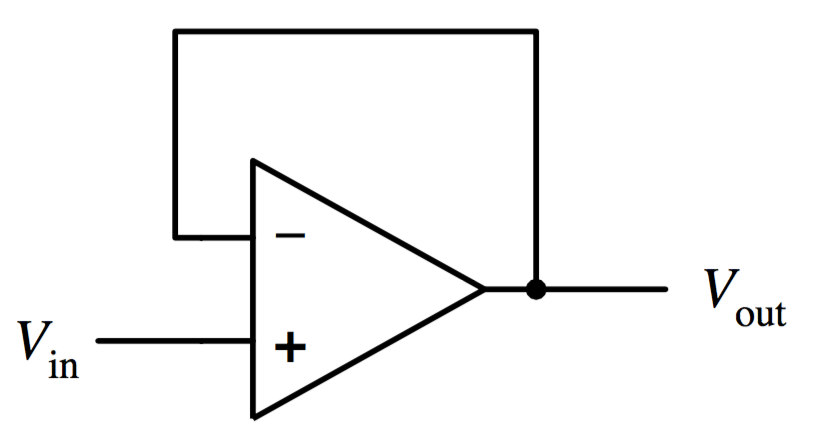
\includegraphics[resolution=300,width=\textwidth/2]{Figure/Introduktion/TilbagekoblingOpAmp.png}
\caption{manglende figurtekst}
\label{fig:TilbagekoblingOpAmp}
\end{figure}
\noindent
%
I eksemplet ovenfor sendes hele udgangssignalet tilbage til den inverterende indgang. Udtrykket for koblingen kan skrives som VOUT = Ao(VIN-fVOUT), hvor f=1, da hele udgangssignalet sendes tilbage til V-. Spædningsforskellen mellem inputterminalerne er 0 i det øjeblik VOUT har samme potentiale som VIN. Opampen forstærker kun forskellen mellem de to spændinger, V+ og V-, som i dette tilfælde hurtigt bliver 0, hvorfor VOUT ikke gå mod uendelig men mod Vin. Med argumentet VOUT=VIN kan udtrykket Ao=VOUT/VIN, skrives som Ao=VOUT/VIN=1, hvilket betyder at forstækningen er 1. Denne kobling kaldes også for en buffer.\\
%
Forstærkningen kan styres ved at det kun er en del af udgangssignalet (VOUT) som sendes tilbage til den inverterende indgang (V-). På den måde vil VOUT forstærkes tilpas nok til at V- får samme potentiale som V+. Dette illustreres i følgende eksempel hvor tilbagekoblingen sker igennem en spændingsdeling.
%
\begin{figure}[H]
\centering
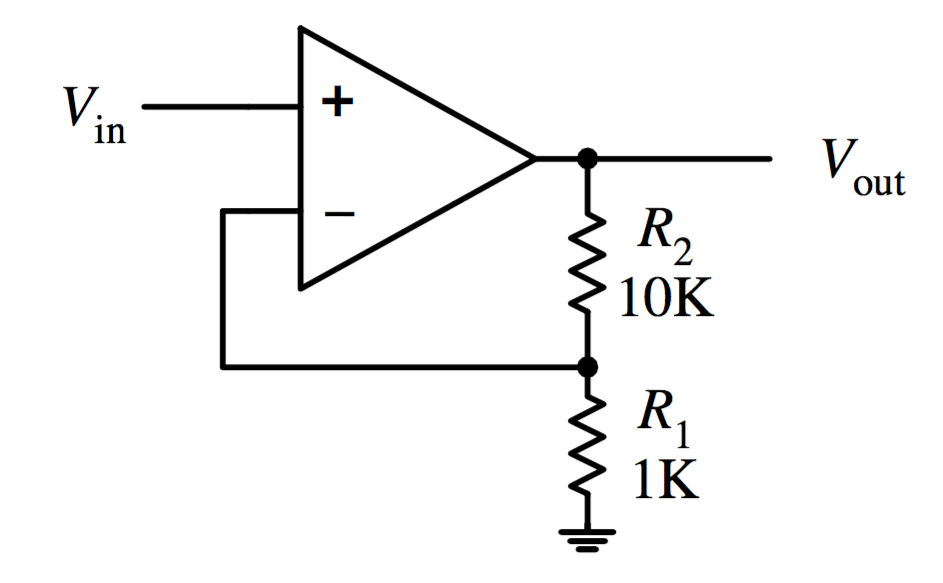
\includegraphics[resolution=300,width=\textwidth/2]{Figure/Introduktion/TilbagekoblingSpaendingsdelingOpAmp.png}
\caption{manglende figurtekst}
\label{fig:TilbagekoblingSpaendingsdelingOpAmp}
\end{figure}
\noindent
%
Spændingsdelingen medfører at $V-=(R1/R1+R2)V_{OUT}$, hvilket i eksemplet kan skrives som $V_-=(1K/1K+10K)V_{OUT}$. V- er altså kun en brøkdel af VOUT. For at V- kan få samme potentiale som V+,må VIN forstærkes indtil VOUT bliver tilpas stor. VOUT skal ifølge udtrykket være 11 gange større end VIN før V- får samme potentiale som V+. Indgangssignalet forstærkes derfor 11 gange, hvilket medfører at udgangssignalet er 11 gange større end indgangssignalet. Udtrykket Ao=VOUT/VIN kan derfor skrives som Ao=11/1=11, hvilket betyder at forstærkingen er 11. (V+-V-)=(VIN-fVOUT)=0 for f=1/11.  
På den måde er det ved hjælp af tilbagekobling, hvor kun en brøkdel af udgangsignalet føres tilbage, muligt at styre hvor meget et signal skal forstærkes i en opamp.\\
%
Ligesom det var muligt at lave en buffer med forstærkningen 1, er det også muligt at lave en inverterende buffer med forstærkningen -1. Dette kan realiseres ved at lave tilbagekoblingen som en del af en spændingsdeler mellem VIN og VOUT, på den inverterende indgang, imens den ikke inverterende indgang (V+) forbindes til ground. Laves en spændingsdeling med to lige store modstande, vil spændingsfaldet være ens over begge modstande, hvorfor der vil ske en halvering af spændingen. Dette er netop grunden til at den inverterende buffer kun invertere signalet uden at forstærke signalet.\\
%
Laves en spændingsdeling med to forskellige størrelser modstande, vil spændingsfaldet afhænge af modstandene. Dette kan ses i eksemplet med den inverterende forstærker herunder.
%
\begin{figure}[H]
\centering
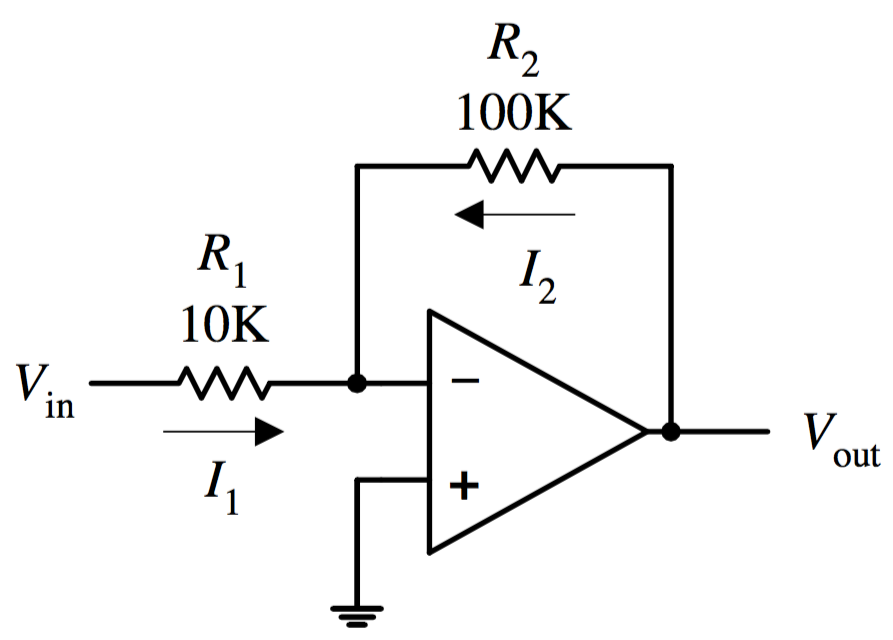
\includegraphics[resolution=300,width=\textwidth/2]{Figure/Introduktion/TilbagekoblingSpaendingsdeling10K100KOpAmp.png}
\caption{manglende figurtekst}
\label{fig:TilbagekoblingSpaendingsdeling10K100KOpAmp}
\end{figure}
\noindent
%
I eksemplet laves en spændingsdeling mellem VIN og VOUT ved hjælp af R1 og R2. Spændingen herimellem danner baggrund for spændingen på den inverterende indgang (V-). Den ikke inverterende indgang (V+) er forbundet til ground, hvilket medfører udtrykket VOUT = Ao(0V-VIN) = -AoVIN. Udtrykket kan også skrives som VOUT/VIN=-Ao hvor -Ao udtrykker forstækningen som resultat af spændingsdelingen mellem R1 og R2. -Ao kan derfor udtrykkes som -R2/R1 og sættes lig med VOUT/VIN. Forstærkningen i eksemplet ovenfor kan derfor udregnes på følgende måde; -Ao=VOUT/VIN= -R2/R1=-100K/10k=-10. VIN forstærkes med andre ord 10 gange. VOUT kan derfor skrives som VOUT =-100K/10k*VIN. På den måde kan en opamp invertere og forstærke med en ønsket faktor, ved hjælp af en spændingsdeling mellem to modstande.\\
%
Dette kan lade sig gøre fordi V+ på opampen er forbundet til ground, hvilket medfører udtrykket (V+-V-)=0 kan skrives som (0V-V-)=0. Udtrykket fortæller at V- har samme potentiale som V+, hvilket kun kan opfyldes ved at V- også er 0V. V- har som udgangspunkt en spænding domineret af VIN, men da opampen invertere og forstærker signalet via en tilbagekobling, kan det siges at potentialet ved VOUT modsvare potentialet ved VIN. Dette kan vises i eksemplet nedenfor hvor en spændingsdeling mellem to spændningsgeneratorer på 1V skaber et potentiale på 0V mellem sig.
%
\begin{figure}[H]
\centering
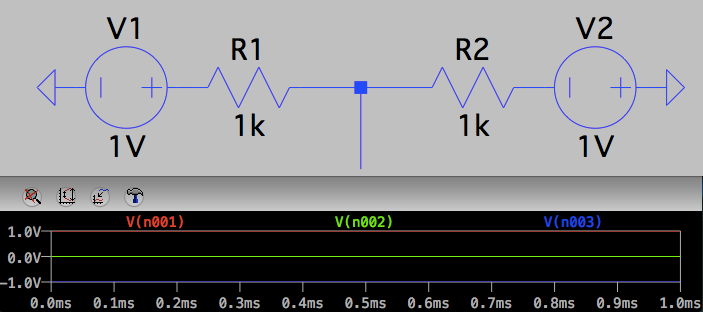
\includegraphics[resolution=300,width=\textwidth]{Figure/Introduktion/PotentialeSpaendingsgeneratorer.png}
\caption{manglende figurtekst}
\label{fig:PotentialeSpaendingsgeneratorer}
\end{figure}
\noindent
%
R1 og R2 er i eksemplet begge 1K Ohm for at spændingsfaldet er ligeligt fordelt over dem. R1 er forbundet til et potentiale på 1V, mens R2 to er forbundet til et potentiale på -1V. Spændningsdelingen mellem modstandene skaber derfor et potentiale på 0V imellem sig, hvilket også kaldes Virtual Ground. Virtual ground skal ikke forveksles med ground, men forstås som en simulering af ground hvor potentialet er 0V.\\
%
Opampen udnytter altså  muligheden for at en spændingsdeling med et positivt potentiale på den ene side og et negativt potentiale på den anden side kan skabe et potentiale på 0V imellem sig. Udtrykket (0V-V-)=0, som fortæller at V- skal have et potentiale svarende til 0V ved V+, kan derfor omskrives til (0V-0V)=0. 
VOUT = Ao(V+-V-)\\
%
SUMMING AMPLIFIER
%
\begin{figure}[H]
\centering
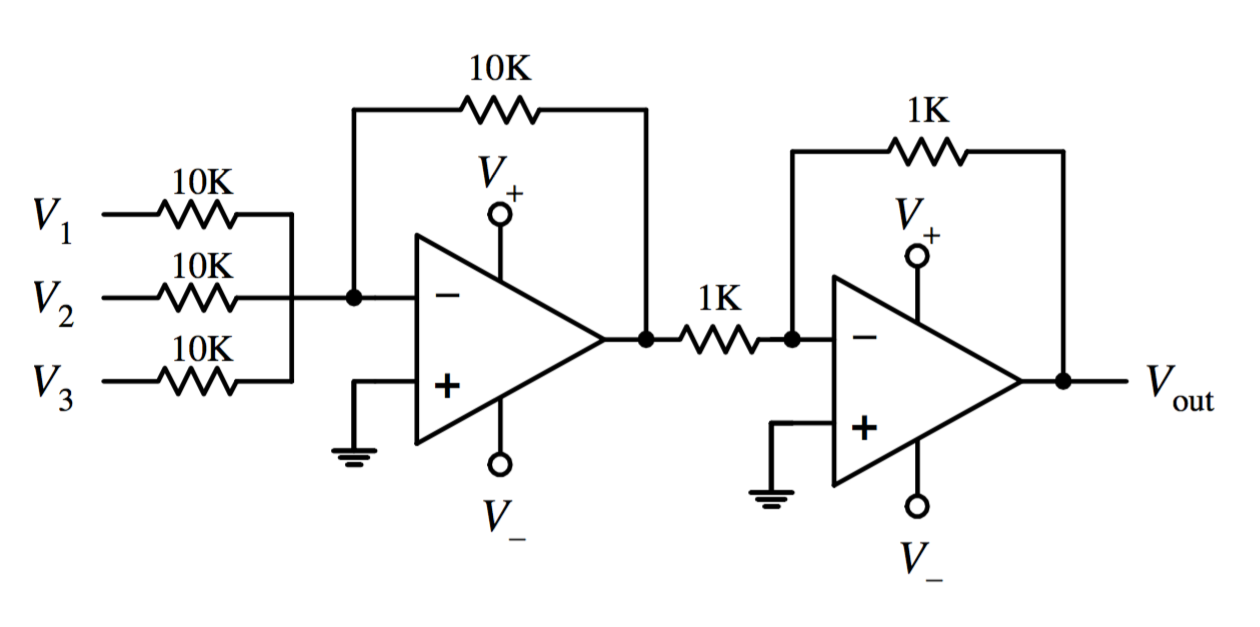
\includegraphics[resolution=300,width=\textwidth]{Figure/Introduktion/SumationskoblingOpAmp.png}
\caption{manglende figurtekst}
\label{fig:SumationskoblingOpAmp}
\end{figure}
\noindent
%